\chapter{Конструкторский раздел}
В данном разделе представлены требования к разрабатываемому ПО и схемы выбранных алгоритмов сортировок.


\section{Требования к ПО}
Выбранные алгоритмы сортировки, должны получать на вход целочисленный массив из N (где $N\in[0:5000]$) элементов и возвращать отсоритрованный по возрастанию массив по месту.


\section{Схемы алгоритмов}
Ниже представлены схемы следующих алгоритмов сортировки:
\begin{itemize}
	\item сортировка пузырьком (рисунок 2.1);
	\item соритровка выбором (рисунок 2.2);
	\item сортировка вставками (рисунок 2.3).
\end{itemize}

\begin{figure}
	\center{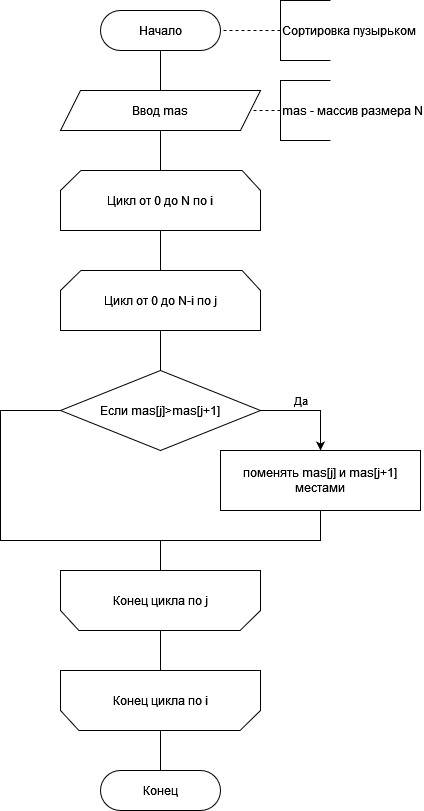
\includegraphics[width=0.8\linewidth]{inc/img/BubbleSort}}
	\caption{Сортировка пузырьком}
\end{figure}

\begin{figure}
	\center{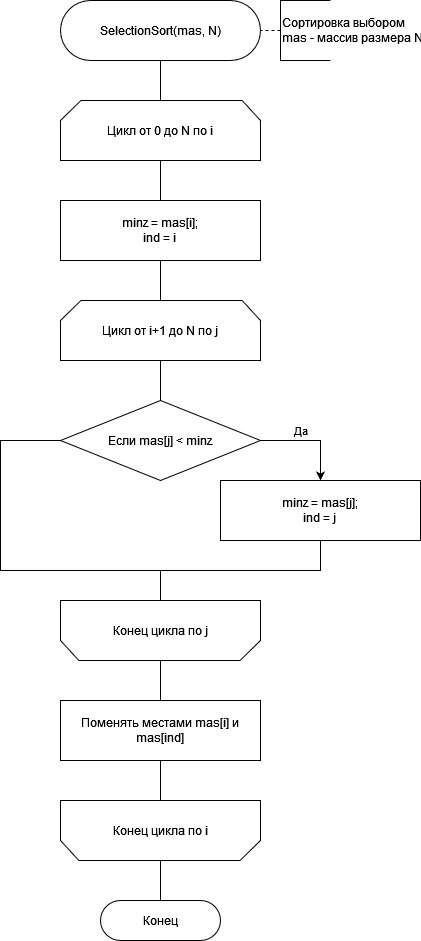
\includegraphics[width=0.6\linewidth]{inc/img/SelectionSort}}
	\caption{Сортировка выбором}
\end{figure}

\begin{figure}
	\center{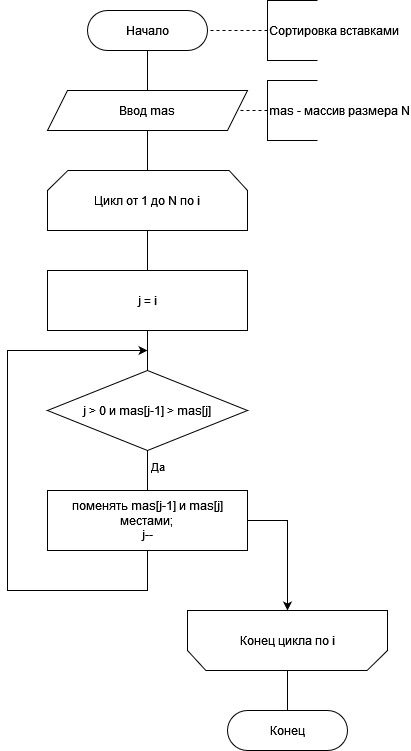
\includegraphics[width=0.8\linewidth]{inc/img/InsertionSort}}
	\caption{Сортировка вставками}
\end{figure}

\newpage
\section{Вывод}
В данном разделе были представлены требования к разрабатываемому ПО и разработаны схемы алгоритмов для выбранных сортировок.